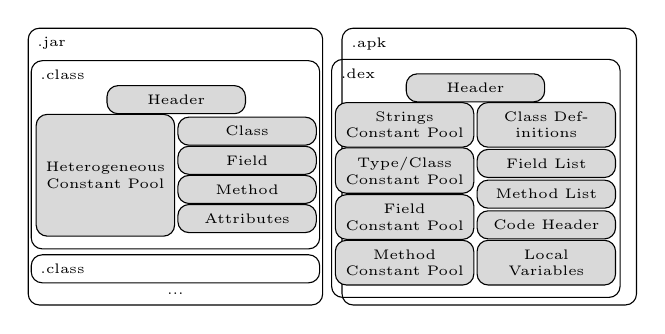
\begin{tikzpicture}[font=\tiny]
  \tikzset{every node/.style={rounded corners}}
  \node[rectangle, draw=black, align=left, text width=1.38in, inner ysep=5em] (jar) at (-.01,-.75){};
  \node[below right] at (jar.north west) {.jar};
  \node[rectangle, draw=black, align=left, text width=1.35in, inner ysep=3.4em] (class) at (-.01,-.6){};
  \node[below right] at (class.north west) {.class};
  \node[rectangle, fill=gray!30, draw=black, align=center, text width=.6in] at (0,.1){Header};
  \node[rectangle, fill=gray!30, draw=black, align=center, text width=.6in, inner ysep=1.73em] at (-.9,-.86){Heterogeneous Constant Pool};
  \node[rectangle, fill=gray!30, draw=black, align=center, text width=.6in] at (.9,-.3){Class};
  \node[rectangle, fill=gray!30, draw=black, align=center, text width=.6in] at (.9,-.67){Field};
  \node[rectangle, fill=gray!30, draw=black, align=center, text width=.6in] at (.9,-1.04){Method};
  \node[rectangle, fill=gray!30, draw=black, align=center, text width=.6in] at (.9,-1.41){Attributes};
  \node[rectangle, draw=black, align=left, text width=1.35in] at ([yshift=-.7em]class.south){.class};
  \node[below] at ([yshift=.8em]jar.south){...};
  
  \node[rectangle, draw=black, align=left, text width=1.38in, inner ysep=5em] (apk) at ([xshift=6em]jar.east){};
  \node[below right] at (apk.north west) {.apk};
  \node[rectangle, draw=black, align=left, text width=1.35in, inner ysep=4.3em] (dex) at (3.805,-.9){};
  \node[below right] at (dex.north west) {.dex};
  \node[rectangle, fill=gray!30, draw=black, align=center, text width=.6in] at (3.8,.25){Header};
  \node[rectangle, fill=gray!30, draw=black, align=center, text width=.6in] at (2.9,-.22){Strings Constant Pool};
  \node[rectangle, fill=gray!30, draw=black, align=center, text width=.6in] at (2.9,-.8){Type/Class Constant Pool};
  \node[rectangle, fill=gray!30, draw=black, align=center, text width=.6in] at (2.9,-1.39){Field\\Constant Pool};
  \node[rectangle, fill=gray!30, draw=black, align=center, text width=.6in] at (2.9,-1.97){Method Constant Pool};
  \node[rectangle, fill=gray!30, draw=black, align=center, text width=.6in] at (4.7,-.22){Class Definitions};
  \node[rectangle, fill=gray!30, draw=black, align=center, text width=.6in] at (4.7,-.71){Field List};
  \node[rectangle, fill=gray!30, draw=black, align=center, text width=.6in] at (4.7,-1.1){Method List};
  \node[rectangle, fill=gray!30, draw=black, align=center, text width=.6in] at (4.7,-1.49){Code Header};
  \node[rectangle, fill=gray!30, draw=black, align=center, text width=.6in] at (4.7,-1.97){Local Variables};
\end{tikzpicture}
